\documentclass[12pt]{article}
\usepackage{../../../lecture_notes}
\usepackage{../../../math}
\usepackage{../../../uark_colors}

\hypersetup{
  colorlinks = true,
  allcolors = ozark_mountains,
  breaklinks = true,
  bookmarksopen = true
}

\newcommand{\answer}[1]{{\color{blue_winged_teal}\textbf{Answer:} #1}}
\newcommand{\pts}[1]{{\color{zinc500}[#1 points]}}

\begin{document}
\begin{center}
  {\Huge\bf Final - Fall 2025}
  
  \smallskip
  {\large\it ECON 4753 — University of Arkansas}
\end{center}

\vspace{5mm}
The following question is based on data collected about faculty at UT Austin and each instructor's average course evaluations. 
There are a total of 463 instructors with 195 being female and 268 being male.
For male instructors the average rating is $\bar{y}_M = 4.07$ and a standard deviation of $\sigma_{y, M} = 0.56$.
For female instructors the average rating is  $\bar{y}_F = 3.90$ and a standard deviation of $\sigma_{y, M} = 0.54$.

Regressing evaluations on an indicator for being a male instructor produces the following output:

  \begin{smallcodeblock}[{}]
OLS estimation, Dep. Var.: eval
Observations: 463
Standard-errors: IID 
             Estimate Std. Error  t value  Pr(>|t|)    
(Intercept)  3.901026   0.039330 99.18747 < 2.2e-16 ***
gender::male 0.168004   0.051695  3.24994 0.0012388 ** 
---
Signif. codes:  0 '***' 0.001 '**' 0.01 '*' 0.05 '.' 0.1 ' ' 1
  \end{smallcodeblock}

\begin{enumerate}
  \item \pts{10} What is the sample distribution of the male-specific sample mean of the evaluation?
  
  \answer{
    $\bar{y}_M \sim \mathcal{N} (\mu_0, 0.56^2 / 268)$
  }
  
  \item \pts{10} Form a 90\% confidence interval around the male specific sample mean (the critical value is $1.65$). Interpret this confidence interval in words.

  \answer{
    $4.07 \pm 1.65 * \sqrt{0.56^2 / 268} = (3.99, 4.15)$. 
    With 90\% confidence, our male average evaluation is between 3.99 and 4.15.
  }
  
  \item \pts{10} Do male and female instructors have different average ratings? Is this difference statistically significant?
  
  \answer{
    Yes, because the coefficient on \texttt{gender::male} is statistically significant. 
  }
\end{enumerate}

\newpage
%% Question on Diamonds' sale price
The following questions are based on data about diamond sales prices and their characteristics. 
For each diamond, we record their cut (Fair, Good, Very Good, Premium, and Ideal) as well as their caret.
For this question, I created bins of caret size: 0--0.5, 0.5--1, 1--2, and 2+ carets.

The regression examines how diamond cut quality affects price while controlling for carat size.

  \begin{smallcodeblock}[{}]
                                 est_lin             est_bin
Dependent Var.:                    price               price
                                                            
Constant             -3,875.5*** (51.16)      121.4* (60.48)
cut = Good            1,120.3*** (55.00)    573.8*** (66.74)
cut = VeryGood        1,510.1*** (52.73)    725.1*** (62.97)
cut = Premium         1,439.1*** (53.21)    697.9*** (63.34)
cut = Ideal           1,800.9*** (51.69)    762.1*** (61.60)
carat                 7,871.1*** (24.88)                    
carat_bin = 0.5<x<=1                      2,005.0*** (10.49)
carat_bin = 1<x<=2                        6,796.1*** (26.58)
carat_bin = x>=2                         14,164.6*** (60.88)
____________________ ___________________ ___________________
  \end{smallcodeblock}


\begin{enumerate}
  \setcounter{enumi}{3}
  \item \pts{10} When modeling the relationship between carat size and diamond price, you could either use carat as a linear term or create bins/categories. 
  What are the advantages and disadvantages of using carat as a linear term versus creating bins (e.g., small, medium, large diamonds)?
  
  \answer{
    Including the caret linearly assumes the change in price per caret is constant as you increase the care size (e.g. going from 0.25 to 0.5 is the same price difference as 1.25 to 1.5).
    The bins allows a more flexible relationship to be estimated (at the cost of being more difficult to explain to stakeholders).
  }

  \bigskip
  \item \pts{5} Consider the regression in the first column (with the linear term for `carat'). 
  Interpret the coefficient on \texttt{Premium} in words. Comment on it's statistical significance.

  \answer{
    Relative to the `Fair' cut diamonds, a `Premium' cut diamond on average is about $1439$ dollars more expensive.
    This difference is statistically significant.
  }
  
  \bigskip
  \item  Consider the regression in the first column (with the linear term for `carat'). The regression controls for carat size when examining the relationship between cut and sales price.
  \begin{enumerate}[label=(\alph*)]
    \item \pts{10} Why is it important to control for carat size when trying to understand the effect of cut quality on diamond prices?

    \answer{
      The caret size and the cut quality are probably positively correlated. 
      This means that our simple regression in column 1 assigns the effect of caret size to the cut quality. 
      Controlling for the caret allows us to seperate the portion that is due to each factor.
    }
    
    \item \pts{5} Interpret the coefficient on carat in words. Include a 95\% confidence interval for this coefficient when interpreting.
    
    \answer{
      Holding fix the cut quality of the diamond, being an extra carat larger is associated with an increased price of about $\$7800$ on average. 
    }
  \end{enumerate}
\end{enumerate}




\newpage
The following questions are based on monthly data on US natural gas consumption in and the average temperature (Fahrenheit) in NYC's central park. 
See the figure and regression table on the next page.

\begin{enumerate}
  \setcounter{enumi}{6}
  \item \pts{10} The time-series data clearly shows seasonal patterns with higher consumption in the winter months. Which term(s) in my time-series regression estimate these patterns?
  
  \answer{The month indicators estiamte the seasonal patterns.}

  \bigskip
  \item \pts{10} The regression includes a continuous \texttt{date} variable to capture the time trend. 
  Interpret the coefficient on \texttt{date} in words. 
  What does it tell us about natural gas consumption over time?
  
  \answer{E
    very additional day that goes by, natural gas consumption is expected to rise by about $0.16$ units. 
    Over the course of a month, this is an increase of about 4.8 units.
    Natural gas consumption is trending up, though relatively weekly given the scale of the outcome variable.
  }

  \bigskip
  \item \pts{10} Interpret the coefficient on \texttt{avg\_temp} in words. 
  
  \answer{For days in a month with a 10 degree higher temperature, the amount of nautral gas consumed is predicted to be about 226 units lower.}
  
  \bigskip
  \item \pts{10} If we remove the \texttt{avg\_temp} term in the regression, the month with the highest natural gas consumption is January. 
  Why do you think controlling for average temperature changed this? 

  \answer{
    Controlling for temperature absorbs the part of the seasonal pattern that is due to it being colder during the winter months. 
    After controlling for temperature, we have removed the influence that had on the seasonal estimates. 
  }
\end{enumerate}



\newpage
\begin{figure}[!th]
  \caption{Natural Gas Consumption and NYC Average Temperature}
  \label{fig:f1}
  
  \vspace*{-2\bigskipamount}
  \begin{center}
    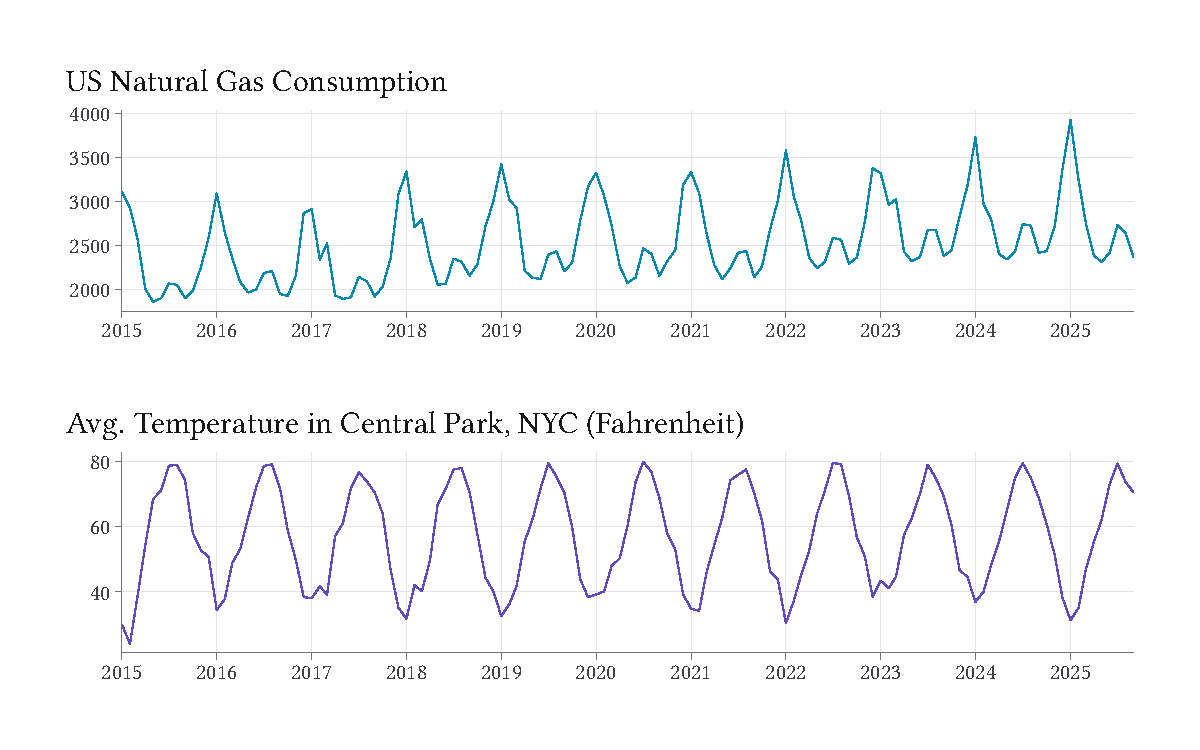
\includegraphics[width = 0.9\textwidth]{figures/p_natural_gas_and_temp.pdf}
  \end{center}
\end{figure}

  \begin{smallcodeblock}[{}]
OLS estimation, Dep. Var.: natural_gas
Observations: 129
Standard-errors: Heteroskedasticity-robust
                               Estimate Std. Error t value   Pr(>|t|)
(Intercept)                     1245.00    1.5e+02    8.33 1.9168e-13 ***
date                               0.16    7.6e-03   21.05  < 2.2e-16 ***
month(date, label = TRUE)::Feb  -410.92    5.2e+01   -7.93 1.5862e-12 ***
month(date, label = TRUE)::Mar  -448.72    6.0e+01   -7.45 1.9206e-11 ***
month(date, label = TRUE)::Apr  -705.47    7.1e+01   -9.98  < 2.2e-16 ***
month(date, label = TRUE)::May  -624.59    9.2e+01   -6.79 5.0866e-10 ***
month(date, label = TRUE)::Jun  -374.43    1.1e+02   -3.32 1.2172e-03 **
month(date, label = TRUE)::Jul    22.44    1.3e+02    0.17 8.6704e-01
month(date, label = TRUE)::Aug   -46.41    1.3e+02   -0.36 7.2256e-01
month(date, label = TRUE)::Sep  -434.92    1.1e+02   -4.01 1.0648e-04 ***
month(date, label = TRUE)::Oct  -589.90    8.4e+01   -7.04 1.4664e-10 ***
month(date, label = TRUE)::Nov  -511.13    6.5e+01   -7.85 2.4482e-12 ***
month(date, label = TRUE)::Dec  -181.61    4.4e+01   -4.11 7.5305e-05 ***
avg_temp                         -22.64    2.8e+00   -8.11 6.2811e-13 ***
  \end{smallcodeblock}



\end{document}
